% *********************************************************************
% © 2026 Jeremy Sylvestre
%
% Permission is granted to copy, distribute and/or modify this document
% under the terms of the GNU Free Documentation License, Version 1.3 or
% any later version published by the Free Software Foundation; with no
% Invariant Sections, no Front-Cover Texts, and no Back-Cover Texts. A
% copy of the license is included in the appendix entitled “GNU Free
% Documentation License” that appears in the output document of this
% PreTeXt source code. All trademarks™ are the registered® marks of
% their respective owners.
%
% *********************************************************************
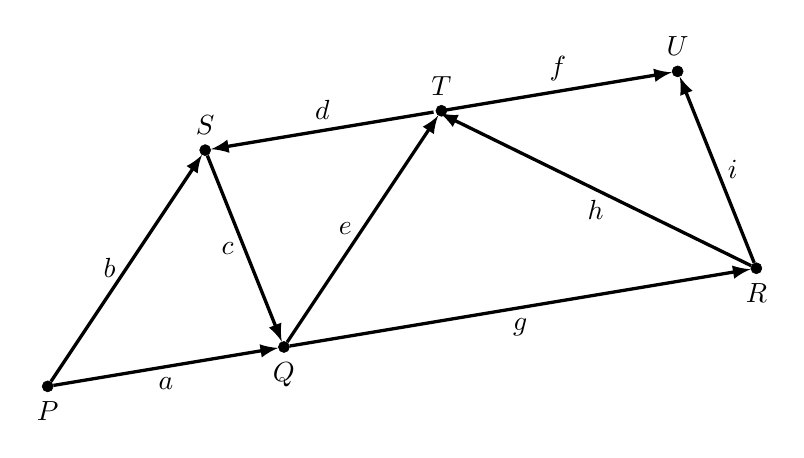
\begin{tikzpicture}[
	point/.style={circle,draw,very thin,fill,inner sep=0pt,minimum size=4pt},
	vector/.style={-latex,very thick},
]

\node[point] (P) at (0,0)   [label=below:$P$] {};
\node[point] (Q) at (3,0.5) [label=below:$Q$] {};
\node[point] (R) at (9,1.5) [label=below:$R$] {};
\node[point] (S) at (2,3)   [label=above:$S$] {};
\node[point] (T) at (5,3.5) [label=above:$T$] {};
\node[point] (U) at (8,4)   [label=above:$U$] {};

\draw[vector] (P) to node[below] {$\uvec{a}$} (Q);
\draw[vector] (P) to node[left ] {$\uvec{b}$} (S);
\draw[vector] (S) to node[left ] {$\uvec{c}$} (Q);
\draw[vector] (Q) to node[left ] {$\uvec{e}$} (T);
\draw[vector] (Q) to node[below] {$\uvec{g}$} (R);
\draw[vector] (R) to node[right] {$\uvec{i}$} (U);
\draw[vector] (R) to node[below] {$\uvec{h}$} ([shift={(-0.02,-0.03)}]T.center);
\draw[vector] ([shift={(-0.1 , -0.0167)}]T.center) to node[above] {$\uvec{d}$} (S);
\draw[vector] ([shift={( 0.03,  0.005 )}]T.center) to node[above] {$\uvec{f}$} (U);

\end{tikzpicture}
